\section{Gerador}

O \texttt{Generator} tem, como função, recebendo parâmetros como comprimento,
largura, raio, etc., gerar ficheiros de texto com a extensão \verb|.3d|, cujo conteúdo
é a informação sobre as figuras a criar. 

Nesta secção ir-se-á descrever o processo de desenvolvimento das figuras
necessárias do sistema solar. As figuras pertinentes a desenhar são a esfera
(para os planetas e sol) e um disco (para alguns planetas que os tenham, como
por exemplo Saturno). 



\subsection{Esfera}
%---------------------------------------------------------------------------------------------------------------%
\subsubsection{Análise do Problema}
Para a construção da esfera teve-se que ter em conta coordenadas esféricas
modificadas para o referencial rodado com Y para cima, Z como eixo das abcissas
e X como eixo das ordenadas, como demonstra a Equação~\ref{eq:equ2}.


\begin{equation}
    \begin{cases}
    x = \cos(\phi) * \sin(\theta) * \rho \\
    y = \sin(\phi) * \rho \\
    z = \cos(\phi) * \cos(\theta) *\rho
    \end{cases}
\label{eq:equ2}
\end{equation}

Na Equação~\ref{eq:equ2}, $\rho$ representa o raio, $\phi$ o ângulo polar sendo
$\phi \in [-\dfrac{\pi}{2}, \dfrac{\pi}{2}]$, $\theta$ representa o ângulo
azimutal sendo $\theta \in [0, 2\pi]$. 


\newpage
\subsubsection{Diagrama}


\begin{center}
 	
 	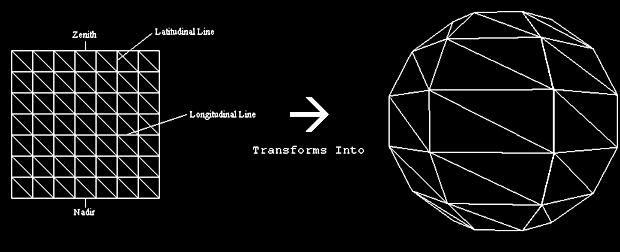
\includegraphics[width=\textwidth,height=\textheight,keepaspectratio]{resources/sphere05.jpg}
 	\captionsetup{type=figure, width=0.8\linewidth}
	\caption{Objetivo do algoritmo de construção de esfera}
\label{fig:ssec1:diagram:plane:to:sphere} 
\end{center}



\begin{center}
 	
 	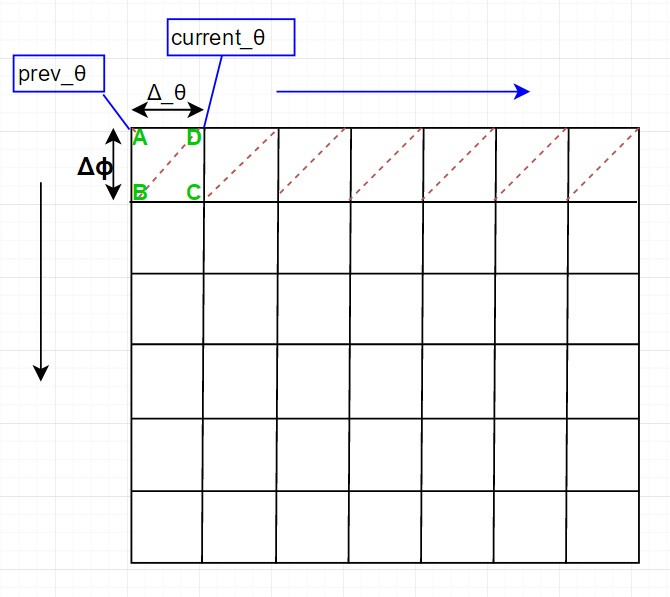
\includegraphics[keepaspectratio]{resources/esferaw.jpg}
 	\captionsetup{type=figure, width=0.8\linewidth}
	\caption{Diagrama de representativo de construção de esfera}
\label{fig:ssec1:diagram:sphere} 
\end{center}


No \emph{Figura~\ref{fig:ssec1:diagram:sphere}} pode-se ver uma matriz, que
representa a esfera nos graus de $\phi$ e $\theta$ para 6 \emph{stacks}
e 7 \emph{slices}. Assim como um mapa representativo da Terra, pretende-se
mostrar os pontos se a esfera fosse aplanada (ver
\emph{Figura~\ref{fig:ssec1:diagram:plane:to:sphere}}).

Em cada quadrícula são calculados 4 pontos iniciais, com base nos cálculos
apresentados pelo fórmula anterior. Note-se que, se usou duas variáveis para
guardar o $\phi$ anterior e o $\phi$ corrente, e $\theta$ anterior  e $\theta$
corrente. Adicionalmente é calculada a diferença de graus entre \emph{slices}
e \emph{stacks}, representados por $\Delta \phi$ e $\Delta \theta$,
respetivamente. 

A intenção é calcular cada quadricula para cada linha e coluna, com auxilio das
diferenças dos ângulos e à medida que se avança em cada quadricula, guardar
o último grau calculado ($\phi$ e $\theta$) e calcular nos pontos com
o incremento nestes ângulos. Assim desloca-se para a direita na matriz, conforme
$\theta$ avança de 0 para $2\pi$ e para baixo, conforme $\phi$ avança de
$\dfrac{\pi}{2}$ para $-\dfrac{\pi}{2}$ (sentido dos ponteiros do relógio).
O \emph{Algoritmo~\ref{alg:secc1:esfera}} representa este processo
e a \emph{Figura~\ref{fig:sec1:sphere:angles}} demonstra o que se
mencionou.  


\begin{center}
 	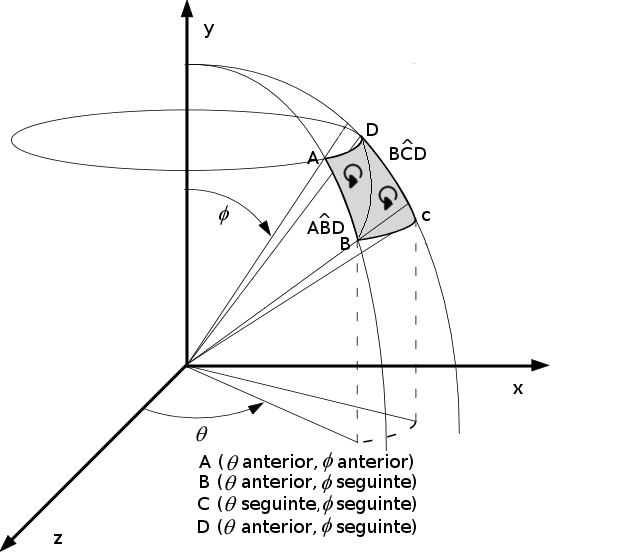
\includegraphics[width=\textwidth,height=0.5\textheight,keepaspectratio]{resources/esfera2.png}
 	\captionsetup{type=figure, width=0.8\linewidth}
	\caption{Diagrama de construção de esfera, com eixos, ordem do vértices
	e ângulos}
\label{fig:sec1:sphere:angles} 
\end{center}

O resultado pode-se ver na \emph{Figura~\ref{fig:ssec1:res:sphere}}, que
demonstra uma esfera em \emph{wireframe} gerada com a aplicação.  

\begin{center}
 	
 	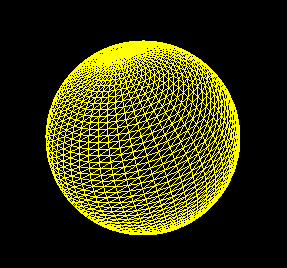
\includegraphics[keepaspectratio]{resources/sphere.png}
 	\captionsetup{type=figure, width=0.8\linewidth}
	\caption{Esfera gerada}
\label{fig:ssec1:res:sphere} 
\end{center}
\newpage

\newgeometry{margin=1cm}
\begin{landscape}
\thispagestyle{empty} %% Remove header and footer.

\begin{algorithm}
\caption{Esfera}\label{alg:secc1:esfera}

\begin{center}
%\footnotesize %% Smaller font size.

\begin{algorithmic}[1]
\State$\Delta\_\theta \gets \dfrac{2\pi}{slices}$

\State$\Delta\_\phi \gets \dfrac{2\pi}{stacks}$

\State$prev\_\phi \gets \dfrac{\pi}{2}$

\State$current\_\phi \gets prev\_\phi - \Delta\_\phi$


\State$i \gets 0$
\While{$i \leq stacks$} 


\State$prev\_\theta \gets 0$
\State$current\_\theta \gets \Delta\_\theta$

\State$j \gets 0$

\While{$j \leq slices$} 


\State$Ponto A \gets raio*\cos(prev\_\phi) * \sin(prev\_\theta)$, $
raio*\sin(prev\_\phi)$, $raio*\cos(prev\_\phi) * \cos(prev\_\theta)$
\State$Ponto B \gets raio*\cos(current\_\phi)*\sin(prev\_\theta)$,$
 raio*\sin(current\_\phi)$,$
 raio*\cos(current\_\phi) * \cos(prev\_\theta)$
\State$Ponto C \gets raio*\cos(prev\_\phi) * 
 \sin(current\_\theta),raio*\sin(prev\_\phi)$,$
 raio*\cos(prev\_\phi) * \cos(current\_\theta)$
\State$Ponto D \gets raio*\cos(current\_\phi) *
 \sin(current\_\theta)$,$raio*\sin(current\_\phi)$,$raio*\cos(current\_\phi) *  \cos(current\_\theta)$
\newline
\State$Triangulo(Ponto A, Ponto B, Ponto D)$ \Comment{Guardado em ficheiro}
\State$Triangulo(Ponto B, Ponto C, Ponto D)$ \Comment{Guardado em ficheiro}
\newline
\State$prev\_\theta \gets current\_\theta$
\State$current\_\theta \gets current\_\theta + \Delta\_\theta $
\newline
\State$j \gets j + 1$ 

\EndWhile{}

\State$prev\_\phi \gets Current\_\phi$
\State$current\_\phi \gets Current\_\phi - \Delta\_\phi $
\State$i \gets i + 1$ 

\EndWhile{}

\end{algorithmic}

\end{center}

\end{algorithm}

\end{landscape}
\restoregeometry{}


\newpage


\subsection{Disco}
Nesta secção descreve os procedimentos usados para desenvolver um disco.
A motivação para o desenvolvimento desta figura provém da necessidade de
representar os anéis que rodeiam os planetas Saturno e Úrano.


\subsubsection{Análise do Problema}

Existem certos elementos do sistema solar, que são característicos de um modelo
do mesmo: anéis e órbitas. Apesar do significado de ambos ser diferente, ambos
podem ser desenhados com o mesmo objeto, variando apenas no raio interno
e externo.

Com efeito, requer-se para este projeto que se criem discos de vários tamanhos
para os anéis de Saturno e Neptuno, e para as órbitas de cada planeta. Note-se
que cada anel tem que ter alguma espessura, uma vez que, num plano, no
\emph{OpenGL} não se consegue ver o objeto. Assim cada disco terá duas
circunferências, uma interior e outra exterior, com raio interno e externo
respetivamente. Assim, as duas circunferências têm os mesmos pontos \emph{xx}
e \emph{zz} mas com uma distancia fixa no eixo \emph{yy}. 

A fórmula para desenhar uma circunferência está representada na
\emph{Equação~\ref{eq:equ3}} 

\begin{equation}
\begin{cases}
			x =  \sin(\theta) * r \\
	    z =  \cos(\theta) * r
\end{cases}
\label{eq:equ3}
\end{equation}



Nesta secção apresentam-se diagramas que explicam o processo de criação de uma
disco.

A \emph{Figura~\ref{fig:ssec1:disc}} representa a forma como a iteração será
feita, bem como apresenta de lado a espessura do disco.


\begin{center}
 	
 	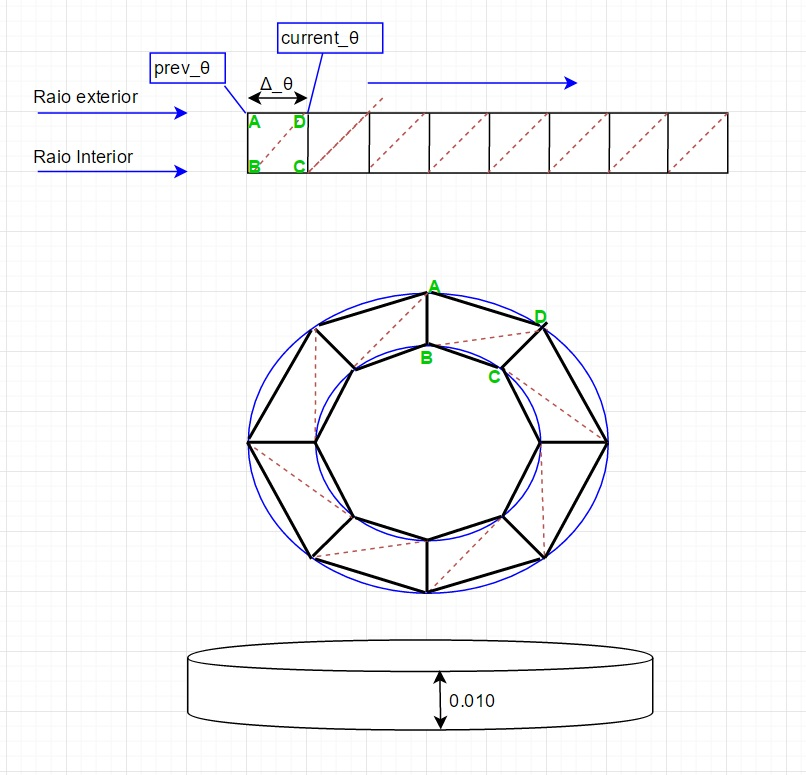
\includegraphics[width=\textwidth,height=\textheight,keepaspectratio]{resources/disco.jpg}
 	\captionsetup{type=figure, width=0.8\linewidth}
	\caption{Diagrama Disco}
\label{fig:ssec1:disc} 
\end{center}

Como se pode verificar o diagrama é relativamente semelhante ao da esfera.
A matriz aqui observada apenas tem uma linha porque não se consideram
\textit{stacks} na representação do disco. As 8 colunas que representam as
8 \textit{slices} (estas 8 slides servem meramente para propósitos
exemplificativos). 


\begin{center}
 	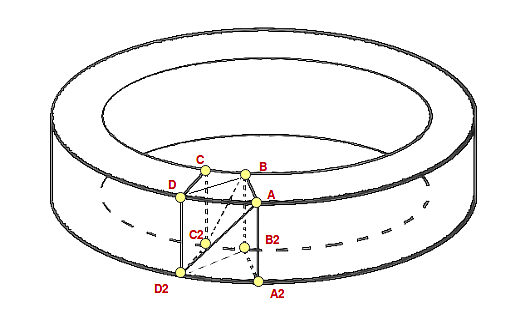
\includegraphics[width=\textwidth,height=0.5\textheight,keepaspectratio]{resources/discodiagram.png}
 	\captionsetup{type=figure, width=0.8\linewidth}
	\caption{Pormenor dos vértices para desenho de um disco}
\label{fig:sec1:disc:vertex} 
\end{center}

Como se pode observar, o raciocínio é desenhar quadricula a quadricula com dois
triângulos cada, neste exemplo verifica-se que a primeira quadricula
é constituída pelos triângulos ABD e BCD.\ As coordenadas de cada ponto (vértice
dos triângulos) são calculados com o auxílio das variáveis angulares
prev\_$\theta $ e current\_$\theta$ usando a formulação das coordenadas
esféricas. A diferença entre esta é o comprimento/largura da quadricula que
corresponde a $\dfrac{2\pi}{slices}$. 

Ora este processo é referente à face superior do disco. Para desenhar a face
inferior faz-se o mesmo processo mas com outros vértices equivalentes nos eixos
\emph{xx} e \emph{zz} mas com uma diferença fixa de 0.010 \emph{yy} para
representar a altura.

Quanto à face lateral do disco o processo é idêntico ao representado na matriz
acima, mas enquanto que, para representar tanto a face superior como a inferior,
os pontos usados têm todos os o mesmo valor \emph{yy}, para representar o lado do disco
usa-se uma combinação dos pontos de ambas as faces. 

Este processo está representado no \emph{Algoritmo~\ref{alg:sec1:disco}},
e um resultado figura na \emph{Figura~\ref{fig:sec1:disc:res1}} e na
\emph{Figura~\ref{fig:sec1:disc:res2}}.  

\begin{center}
 	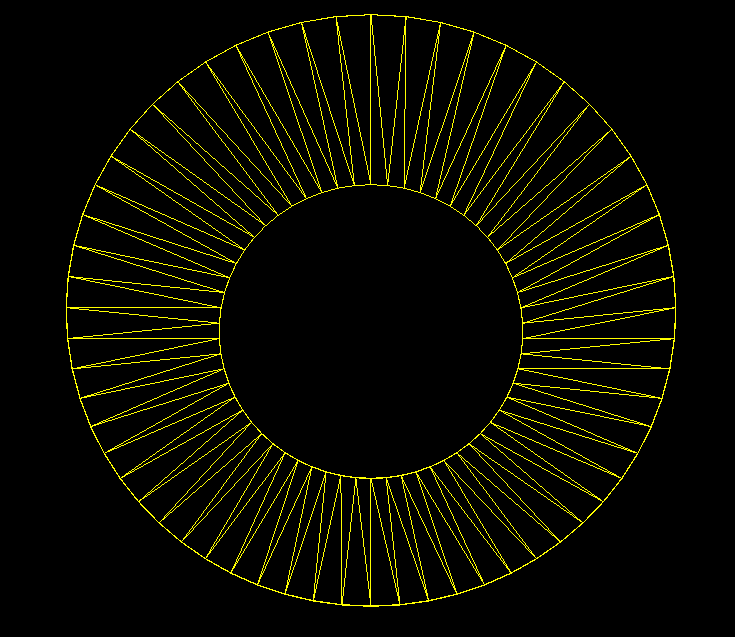
\includegraphics[width=\textwidth,height=0.5\textheight,keepaspectratio]{resources/disco1.png}
 	\captionsetup{type=figure, width=0.8\linewidth}
	\caption{Resultado de um disco em \emph{wireframe}, visto de baixo}
\label{fig:sec1:disc:res1} 
\end{center}


\begin{center}
 	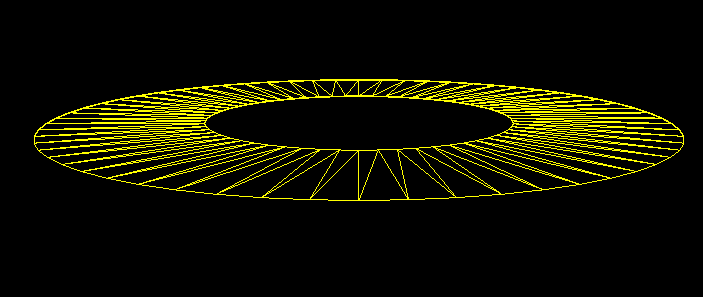
\includegraphics[width=\textwidth,height=0.5\textheight,keepaspectratio]{resources/disco2.png}
 	\captionsetup{type=figure, width=0.8\linewidth}
	\caption{Resultado de um disco em \emph{wireframe}, visto de outro ângulo}
\label{fig:sec1:disc:res2} 
\end{center}




\newgeometry{margin=1cm}
\begin{landscape}
\thispagestyle{empty} %% Remove header and footer.
\begin{algorithm}
\caption{Disco}\label{alg:sec1:disco}

\begin{center}
%\footnotesize %% Smaller font size.

\begin{algorithmic}[1]
\State$\Delta\_\theta \gets \dfrac{2\pi}{slices}$


\State$prev\_\theta \gets 0$
\State$current\_\theta \gets \Delta\_\theta$

\State$i \gets 0$


\While{$i \leq slices$} 

\State$Ponto A \gets raioOut*\sin(prev\_\theta),
 0.005,
 raioOut*\cos(prev\_\theta)$

\State$Ponto B \gets raioIn*\sin(prev\_\theta),
 0.005,
 raioIn*\cos(prev\_\theta)$

\State$Ponto C \gets raioIn*\sin(current\_\theta),
 0.005,
 raioIn*\cos(current\_\theta)$

\State$Ponto D \gets raioOut*\sin(current\_\theta),
  0.005,
 raioOut*\cos(current\_\theta)$

\State$Ponto A2 \gets raioOut*\sin(prev\_\theta),
 -0.005,
 raioOut*\cos(prev\_\theta)$

\State$Ponto B2 \gets raioIn*\sin(prev\_\theta),
 -0.005,
 raioIn*\cos(prev\_\theta)$

\State$Ponto C2 \gets raioIn*\sin(current\_\theta),
 -0.005,
 raioIn*\cos(current\_\theta)$

\State$Ponto D2 \gets raioOut*\sin(current\_\theta),
  -0.005,
 raioOut*\cos(current\_\theta)$




\Comment{Lado de cima}

\State$Triangulo(Ponto D, Ponto B, Ponto A)$ \Comment{Guardado em ficheiro}
\State$Triangulo(Ponto C, Ponto B, Ponto D)$ \Comment{Guardado em ficheiro}



\Comment{Lado de baixo}
\State$Triangulo(Ponto A2, Ponto B2, Ponto D2)$ \Comment{Guardado em ficheiro}
\State$Triangulo(Ponto D2, Ponto B2, Ponto C2)$   \Comment{Guardado em ficheiro}
		  
\Comment{Lado de externo}
\State$Triangulo(Ponto A2, Ponto A, Ponto D2)$\Comment{Guardado em
ficheiro}
\State$Triangulo(Ponto D, Ponto D2, Ponto A)$\Comment{Guardado em
ficheiro}
  
\Comment{Lado de interno}
\State$Triangulo(Ponto B, Ponto C2, Ponto B2)$\Comment{Guardado em
ficheiro}
\State$Triangulo(Ponto C, Ponto C2, Ponto B)$\Comment{Guardado em
ficheiro}



\State$prev\_\theta \gets current\_\theta$
\State$current\_\theta \gets current\_\theta + \Delta\_\theta$

\State$i \gets i + 1$


\EndWhile{}
\end{algorithmic}
\end{center}

\end{algorithm}


\end{landscape}
\restoregeometry{}

\subsection{\emph{Patch} de Bézier baseado em ficheiro de pontos de controlo}

\subsubsection{Análise do Problema}

Para este projeto, requere-se que se obtenha pontos de controlo de uma
superfície de Bézier, através de uma ficheiro \emph{teapot.patch}, para
a construção de um bule de chá, para a representação de um cometa. O formato de
ficheiro é o que se segue:
\begin{enumerate}
	\item Número de \emph{patches};
	\item Índices para \emph{patches} (16 por linha, tantas linhas como nº de
		\emph{patches});
	\item Número de pontos de controlo;
	\item Ponto de controlo (coord.\ x, y, z) por linha, tantas linhas como nº de
		pontos de controlo;
\end{enumerate}

Para armazenar os dados do ficheiro, criou-se uma estrutura com dois valores
inteiros (nº \emph{patches} e nº de pontos), um vetor de vetores de inteiros,
para armazenar os valores dos índices e um vetor de \texttt{Point3d} para
armazenar os pontos de controlo. Além do mais, requere-se que se passe um valor
de tecelagem (\emph{tesselation}), para controlo da malha a criar.

A função de leitura separa o \emph{parsing} de cada elemento no formato descrito
atrás à custa de uma \emph{flag}. Note-se que o ficheiro original tinha os todos
os valores separados por vírgulas, pelo que, por uma questão de eficiência,
removeram-se as vírgulas, deixando os valores separados por espaços. Deste modo,
é possível utilizar as funcionalidades da linguagem de programação em uso
\texttt{C++} e saltar espaços a ler o ficheiro. Uma outra nota sobre o uso de
funcionalidades da linguagem, dado que se está a usar \texttt{vector} para
armazenamento de pontos e índices, o nº de \emph{patches} e o nº de pontos,
recebidos do ficheiro não são utilizados.  

Além do mais, por uma questão de legibilidade e facilidade de manutenção do
código, foram criados dois tipos de dados (\texttt{MatrixF} e \texttt{MatrixP},
escalares de vírgula flutuante e pontos 3D), criados às custas de vetores de
vetores, para guardar valores na forma matricial. Com efeito, uma
\texttt{MatrixP} guarda os pontos de controlo de uma superfície de Bézier
(matriz de pontos 4 $\times$ 4). 

A função \texttt{drawPatch}, trata do processamento de leitura de transformação
dos valores lidos em ficheiro num vetor de \texttt{MatrixP}, onde por último,
para cada matriz armazenada no vetor anterior, para um valor de $i$ e um valor
de $j$ dividido pela tecelagem, iterando cada um desses valor entre 0 e o valor
da tecelagem, cria-se 4 pontos da superfície de Bézier, para cada iteração, que
formem uma quadricula conforme mostra a \emph{Figura~\ref{}}, onde são retirados
os triângulos e armazenados num ficheiro \.3d, todos os vértices calculados.
Para calcular cada ponto da superfície de Bézier, é utilizada a função
\texttt{getBezierPatchPoint}, que recebe um valor de $u$, $v$ e uma matriz de
pontos de controlo. 

\paragraph{Curvas de Bézier}

Uma curva Bézier pode ser definida por um qualquer numero de pontos, pontos
estes chamados pontos de controlo da curva. Transformações como translação
e rotação podem ser aplicadas na curva manipulando estes pontos. 

O algoritmo de \emph{De Casteljeau} oferece uma forma de calcular uma curva,
baseada em 4 pontos de controlo, onde um parâmetro $t \in [0,1]$ varia, e um
ponto é obtido $t$ e $1-t$ entre cada reta de cada ponto de controlo. Cada ponto
intermédio (3 pontos em simultâneo, um em cada reta, para cada variação de $t$),
conecta com cada um dos 3 pontos anteriormente mencionados, criando duas retas
com $t$ a variar de igual modo, nas retas como nas retas dos pontos iniciais. Em
seguida, para cada variação de $t$ das duas retas, dois pontos intersetam-se, e,
por último, para cada variação de $t$, nesta última reta, temos um ponto da
curva de Bézier. Note-se que $t$ varia em simultâneo, para todas as retas
iniciais e intermédias. A \emph{Figura~\ref{fig:casteljeaut}},
e \emph{Figura~\ref{fig:casteljeautree}} ilustram esta explicação.  

\begin{center}	
 	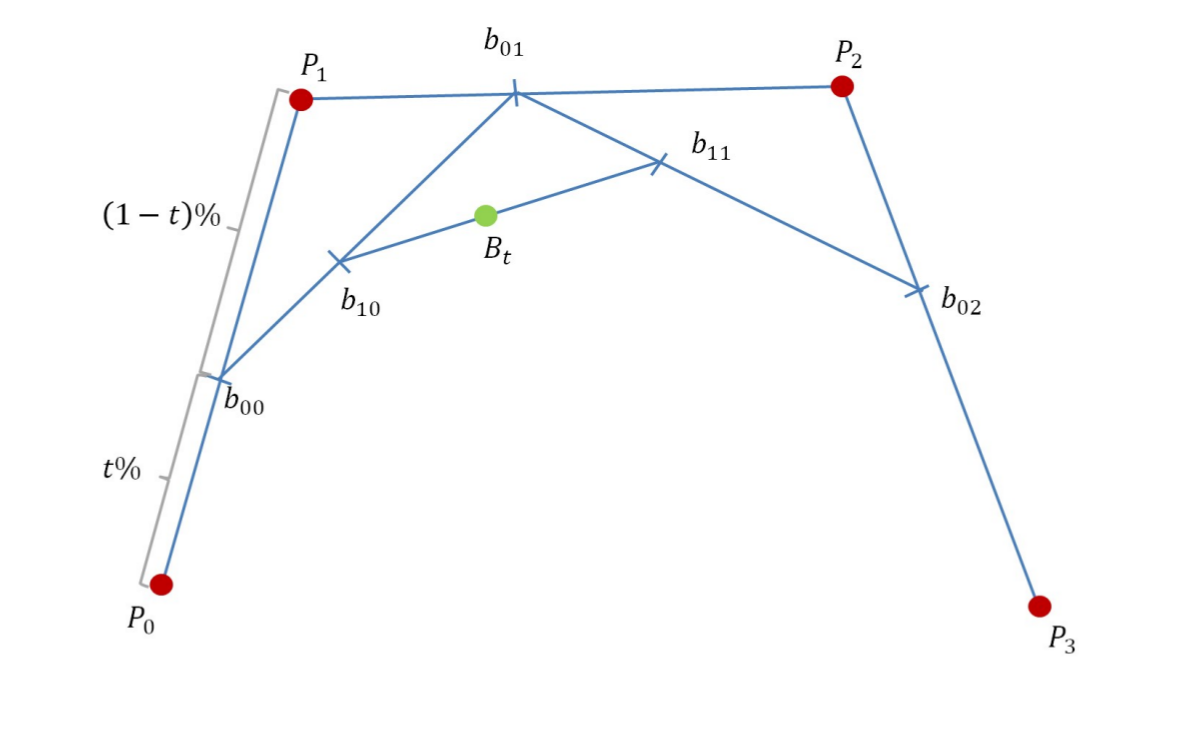
\includegraphics[width=\textwidth,height=\textheight,keepaspectratio]{resources/casteljou.png}
 	\captionsetup{type=figure, width=0.8\linewidth}
	\caption{Algoritmo geométrico \emph{De Casteljeau}}
\label{fig:casteljeaut} 
\end{center}


\begin{center}	
 	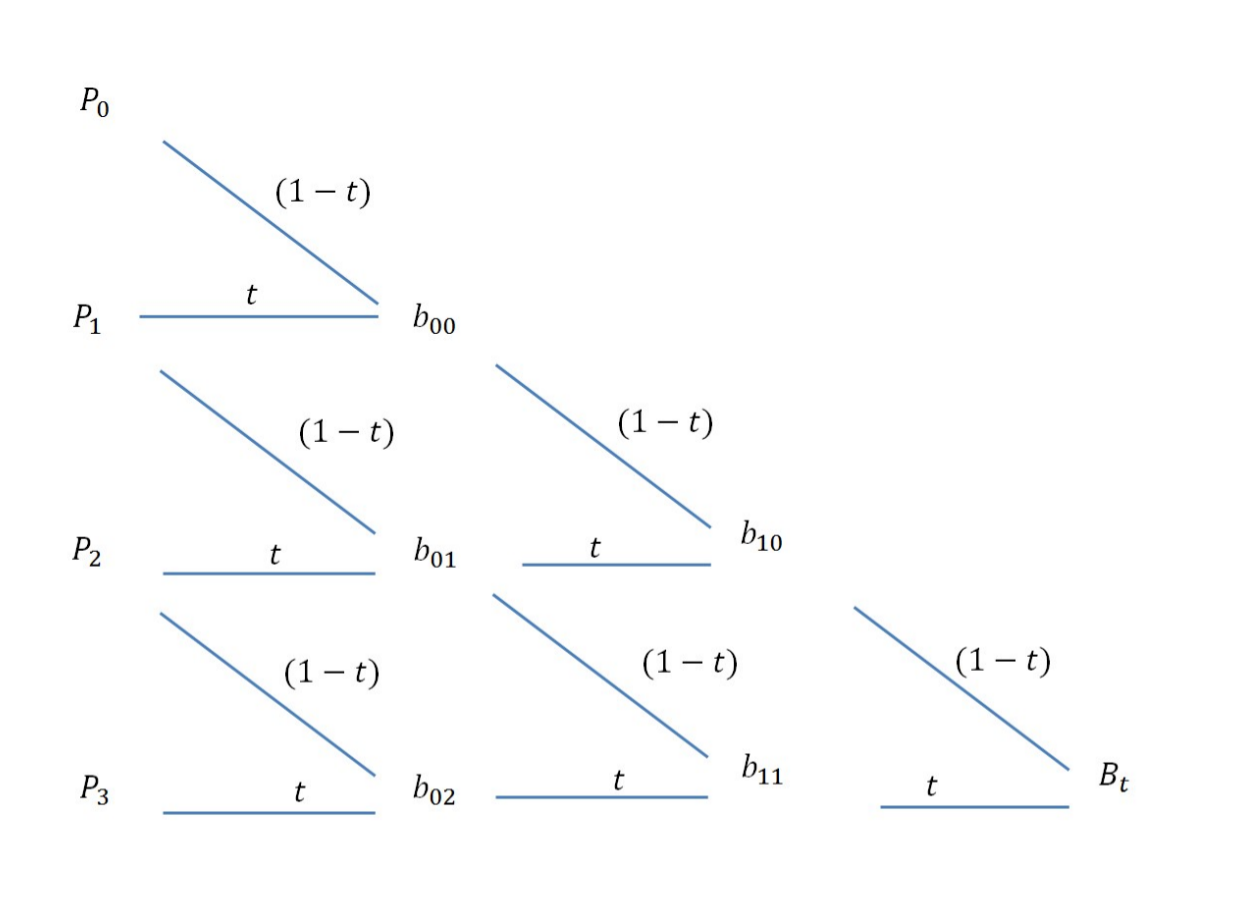
\includegraphics[width=\textwidth,height=\textheight,keepaspectratio]{resources/casteljeau2.png}
 	\captionsetup{type=figure, width=0.8\linewidth}
	\caption{Representação da iteração em cada reta entre pontos referente
		à \emph{Figura~\ref{fig:casteljeaut}}}
\label{fig:casteljeautree} 
\end{center}

A partir da \emph{Figura~\ref{fig:casteljeautree}} é derivada
a \emph{Equação~\ref{eq:beziercurve}}.

\begin{equation}
B(t)=t^{3}P_{3}+3t^{2}(1-t)P_{2}+3t{(1-t)}^{2}P_{1}+{(1-t)}^{3}P_{0}
\label{eq:beziercurve}
\end{equation}

De uma forma mais condensada, a equação anterior pode ser representada como na
\emph{Equação~\ref{eq:beziercurvecondensed}} 


\begin{equation}
B(t)=\sum_{k=0}^{3}B_{3,k}(t)P_{k}
\label{eq:beziercurvecondensed}
\end{equation}


Note-se que a equação anterior é uma particularização de curva cúbica de Bézier,
podendo uma curva de Bézier, ter $n$ graus  onde n corresponde a ($\text{nº
pontos de controlo} - 1$), e $t \in [0,1]$ e o seu somatório é sempre igual a 1,
tomando a forma genérica da \emph{Equação~\ref{eq:beziercurvegenerica}}. 


\begin{equation}
B(t)=\sum_{k=0}^{n}B_{n,k}(t)P_{k}
\label{eq:beziercurvegenerica}
\end{equation}

\begin{center}
 	
 	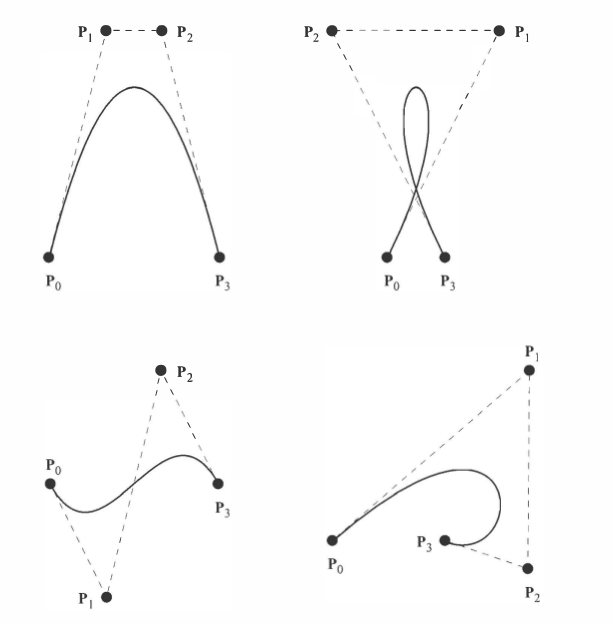
\includegraphics[scale=0.5,keepaspectratio]{resources/exemplos1Bezier.png}
 	\captionsetup{type=figure, width=0.8\linewidth}
	\caption{Curvas exemplo de Bézier}
\label{fig:beziercubicexamples} 
\end{center}


A \emph{Equação~\ref{eq:beziercurve}} pode ser representada na forma matricial
segundo a \emph{Equação~\ref{eq:beziercurvematrix}}. 

\begin{equation}
B(t)= \begin{bmatrix}
       t^{3} & t^{2} & t & 1          
		\end{bmatrix}
		\begin{bmatrix}
		       -1 & 3 & -3  & 1 \\
		        3 & -6 &  3 & 0 \\
		       -3 & 3 & 0 & 0   \\
		        1 & 0 & 0 & 0
		\end{bmatrix}
		 \begin{bmatrix}
		       P_{0}   \\
		       P_{1}   \\
		       P_{2}   \\
		       P_{3}
		     \end{bmatrix}
\label{eq:beziercurvematrix}
\end{equation}

\newpage
\paragraph{Superfícies de Bézier (\emph{patches} de Bézier)}

Se se tiver um \emph{array} bi-dimensional de pontos
$P_{i,j}$, com $i\in[0, m]$, e $j\in[0,n]$, então pode-se
construir uma superfície Bézier da mesma forma usando um método similar a uma
curva cúbica de Bézier. Neste caso, ao invés de um parâmetro, existem dois
($u$ e $v$), onde $u\in[0,1]$ e $v\in[0,1]$.
Uma superfície de Bézier bi-cúbica (m=n=3), dado que tem por base curvas cúbicas
de Bézier definidas por 4 pontos de controlo, uma vez que é bi-dimensional, é definida por 16 pontos de
controlo $P_{i,j}$, e  representa-se pela \emph{Equação~\ref{eq:bezierpatch}}. Um
exemplo de uma superfície de Bézier está na \emph{Figura~\ref{fig:patchexample}} 

\begin{equation}
B(u,v)=\sum_{j=0}^{3}\sum_{i=0}^{3}B_{i}(u)P_{i,j}B{j}(v)
\label{eq:bezierpatch}
\end{equation}



\begin{center}
 	
 	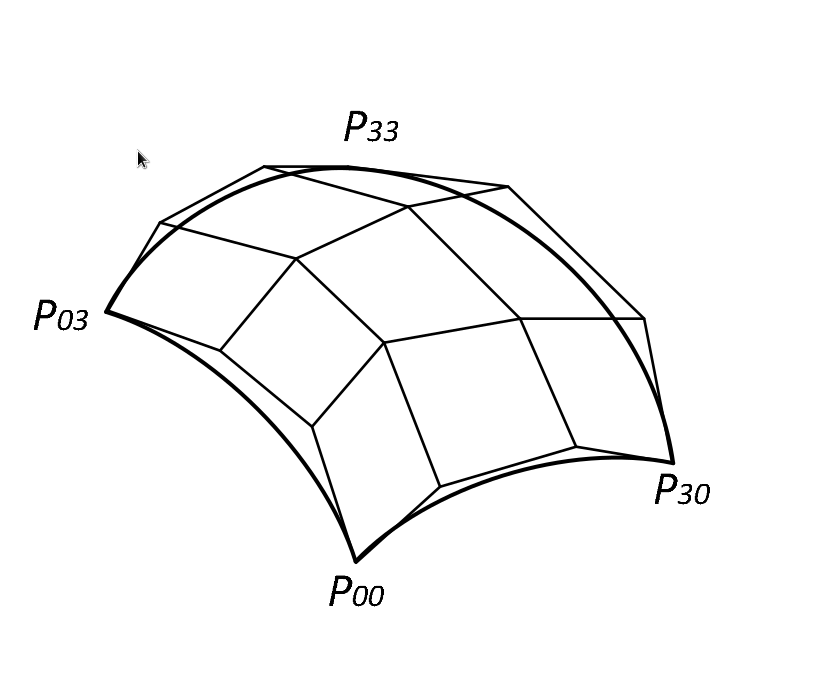
\includegraphics[width=0.5\textwidth,height=0.5\textheight,keepaspectratio]{resources/beziersupf.png}
 	\captionsetup{type=figure, width=0.8\linewidth}
	\caption{Superfície de Bézier bi-cúbica}
\label{fig:patchexample} 
\end{center}
Temos que:
\begin{gather*}
M = \begin{bmatrix}
-1 &  3 & -3 & 1  \\
 3 & -6 & 3  & 0  \\
-3 &  3 & 0  & 0  \\
1  &  0 & 0  & 0  \\
\end{bmatrix}
\end{gather*}

O parâmetros $u$ e $v$ estão entre 0 e 1, à semelhança do parâmetro $t$ da
função para uma curva de Bézier, onde $M$ é a matriz dos coeficientes obtida da
\emph{Equação~\ref{eq:beziercurve}}. A explicação para a obtenção de um ponto
numa superfície de Bézier, e, grosso modo, análoga à obtenção de um ponto numa
curva de Bézier, sendo que neste caso, estão dois parâmetros a variar entre
0 e 1, criando uma malha de com curvas de Bézier, conforme está na
\emph{Figura~\ref{fig:patchexample}}. Derivando
a \emph{Equação~\ref{eq:bezierpatch}} obtém-se
a representação matricial na \emph{Equação~\ref{eq:bezierpatchmatrix}}.

\begin{equation}
B(u,v) = \begin{bmatrix}
       u^{4} & u^{2} & u & 1          \\
		\end{bmatrix}
		M\begin{bmatrix}
		       P_{00} & P_{01} & P_{02} & P_{03}   \\
		       P_{10} & P_{11} & P_{12} & P_{13}   \\
		       P_{20} & P_{21} & P_{22} & P_{23}   \\
		       P_{30} & P_{31} & P_{32} & P_{33}
		     \end{bmatrix}
		M^{T} \begin{bmatrix}
		       v^{3} \\
		       v^{2} \\
		       v^{1} \\
		       v^{0}
		     \end{bmatrix}
\label{eq:bezierpatchmatrix}				 
\end{equation}

\paragraph{Função \texttt{getBezierPatchPoint}}

Antes de descrever a função \texttt{getBezierPatchPoint} é necessário descrever
algumas funções cridas par utilizar nessa função. 

Para cálculos com valores escalares de vírgula flutuante, nomeadamente
multiplicação de matrizes, criou-se a função \texttt{multMatrix} que multiplica
duas matrizes. Para obter um cálculo correto, são obtidas as dimensões das
matrizes (nº de linhas e nº de colunas), tal que, as dimensões para uma dada
matriz M1 são m $\times$ n, e as dimensões para uma dada 
matriz M2 são p $\times$ q. Para obtenção da matriz resultado, tem-se em conta
o nº de linhas da matriz M1 (m) e o nº de colunas da matriz M2 (q), onde
a matriz resultante terá um dimensão m $\times$ q. Note-se que os valores n ---
nº de colunas da matriz M1 --- e p --- nº de linhas da matriz M2 têm que ser
iguais. No entanto, essa verificação não é feita no código, no entanto,
assume-se que o programador sabe da especificação desta função. Para guardar
o valor da multiplicação de matrizes (somatório da multiplicação das linhas com
as colunas), usa-se um acumulador de resultado, fazendo variar um índice k,
entre 0 e p (que poderia ser n).

A função \texttt{matrixPointToScalar} obtém as coordenadas de x, ou de y, ou de
z, da matriz de pontos de controlo e armazena esses valores numa matriz de
escalares.


A função \texttt{getBezierPatchPoint} utiliza
a \emph{Equação~\ref{eq:bezierpatchmatrix}}, sendo o código amigável na sua
leitura e interpretação, uma vez que abstrai detalhes de implementação através
dos tipos de matrizes já mencionados. Em primeiro lugar,  a função calcula
a matriz U e a matriz V, com os parâmetros $u$ e $v$ respetivos, conforme
a equação. A segunda parte do algoritmo é multiplicar a matriz U por M, e matriz
$M^T$ por V e guarda cada resultado numa matriz. Note-se que, $M = M^T$, então
a matriz M é reutilizada.

Para calcular o ponto da superfície de Bézier, é necessário obter cada
coordenada dos pontos de controlo, sendo que a matriz de escalares da coordenada
x será para calcular a coordenada x do ponto da superfície, a matriz de
escalares da coordenada y será para calcular a coordenada y do ponto da
superfície e  a matriz de escalares da coordenada z será para calcular
a coordenada z do ponto da superfície. Cada matriz de escalares é multiplicada
pelo resultado de $UM$, e o resultado desta, com o resultado de $M^{T}V$ ou $MV$.
As matrizes resultantes destas operações são matrizes com dimensão $1\times1$,
com cada valor da coordenada x, y e z do ponto da superfície. Essas coordenadas
são guardadas num \texttt{Point3d} que é retornado pela função. 

Os resultados da aplicação do algoritmo para uma tecelagem de 50 podem ser
vistos nas figuras abaixo.

\begin{center}	
 	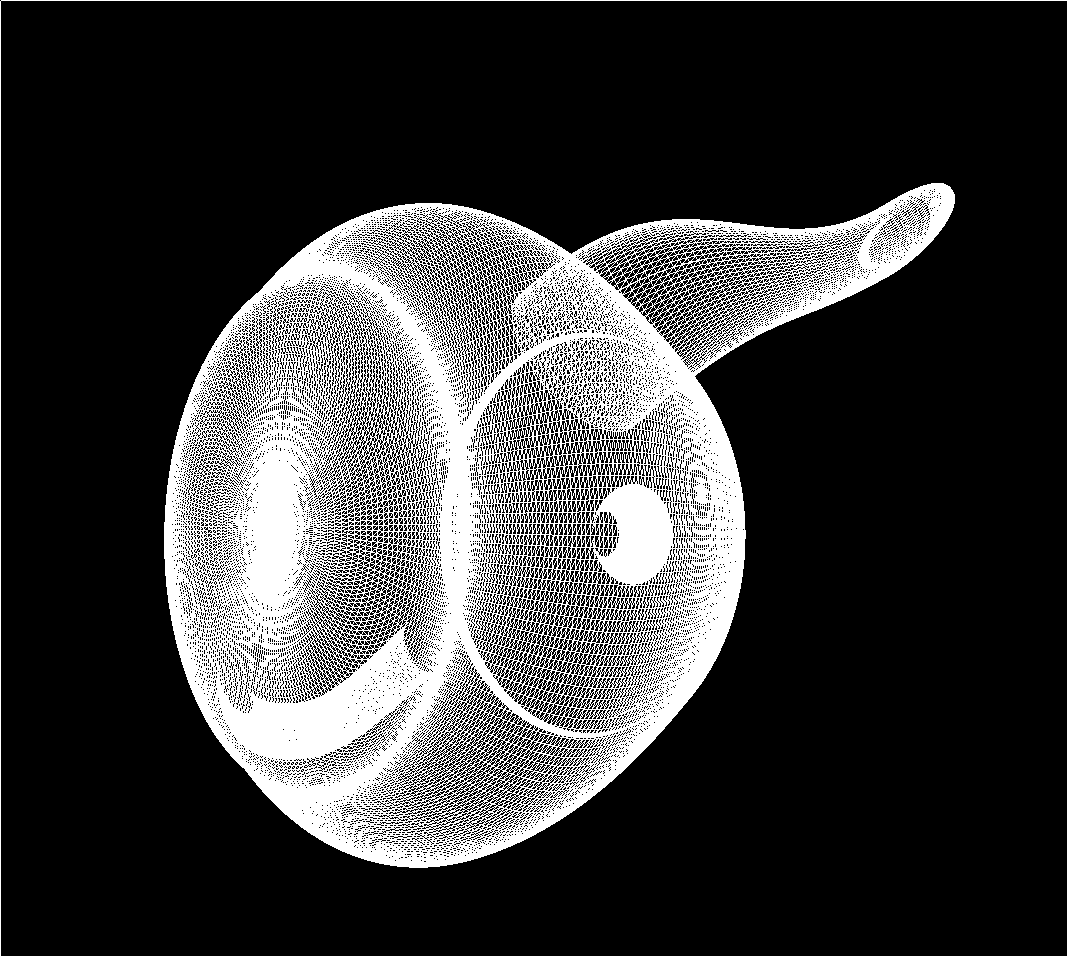
\includegraphics[width=\textwidth,height=\textheight,keepaspectratio]{resources/teapotBaixo.png}
 	\captionsetup{type=figure, width=0.8\linewidth}
	\caption{Bule visto de baixo}
\label{fig:teapotbottom} 
\end{center}

\begin{center}	
 	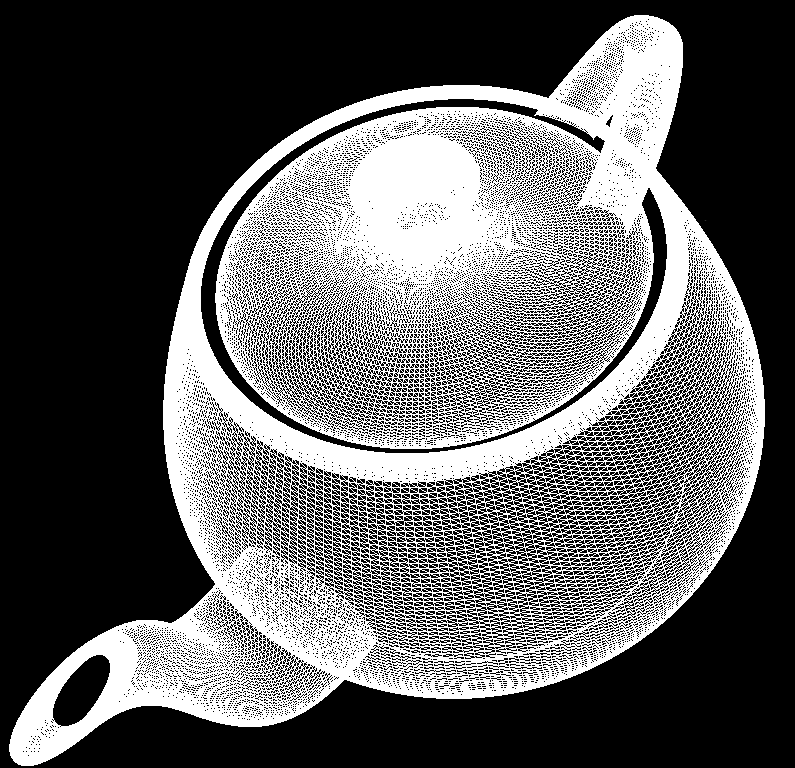
\includegraphics[width=\textwidth,height=\textheight,keepaspectratio]{resources/teapotCima.png}
 	\captionsetup{type=figure, width=0.8\linewidth}
	\caption{Bule visto de cima}
\label{fig:teapotabove} 
\end{center}


\begin{center}	
 	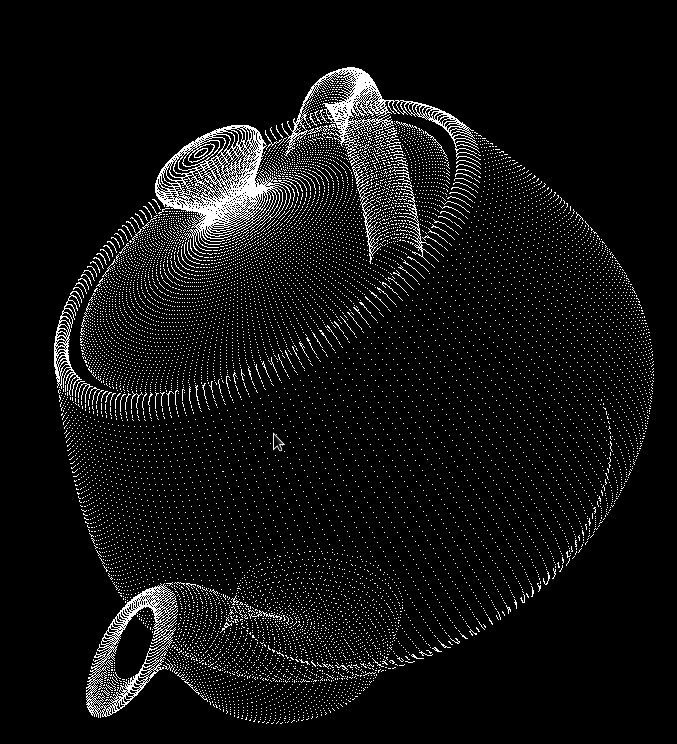
\includegraphics[width=\textwidth,height=\textheight,keepaspectratio]{resources/teapotPontos}
 	\captionsetup{type=figure, width=0.8\linewidth}
	\caption{Pontos da superfície do bule}
\label{fig:teapotpoints} 
\end{center}



